\section{Class Diagram}

The class diagram represents the core domain model and architectural components of the Smart Parking IoT system. The diagram shows 23 classes organized into domain entities, services, controllers, and supporting types.

\subsection{Class Diagram Overview}

\begin{figure}[H]
\centering
\href{https://drive.google.com/file/d/1pyrfXCZQ7EooY92Xx5RG6gMXaX-m-0xJ/view?usp=sharing}{%
  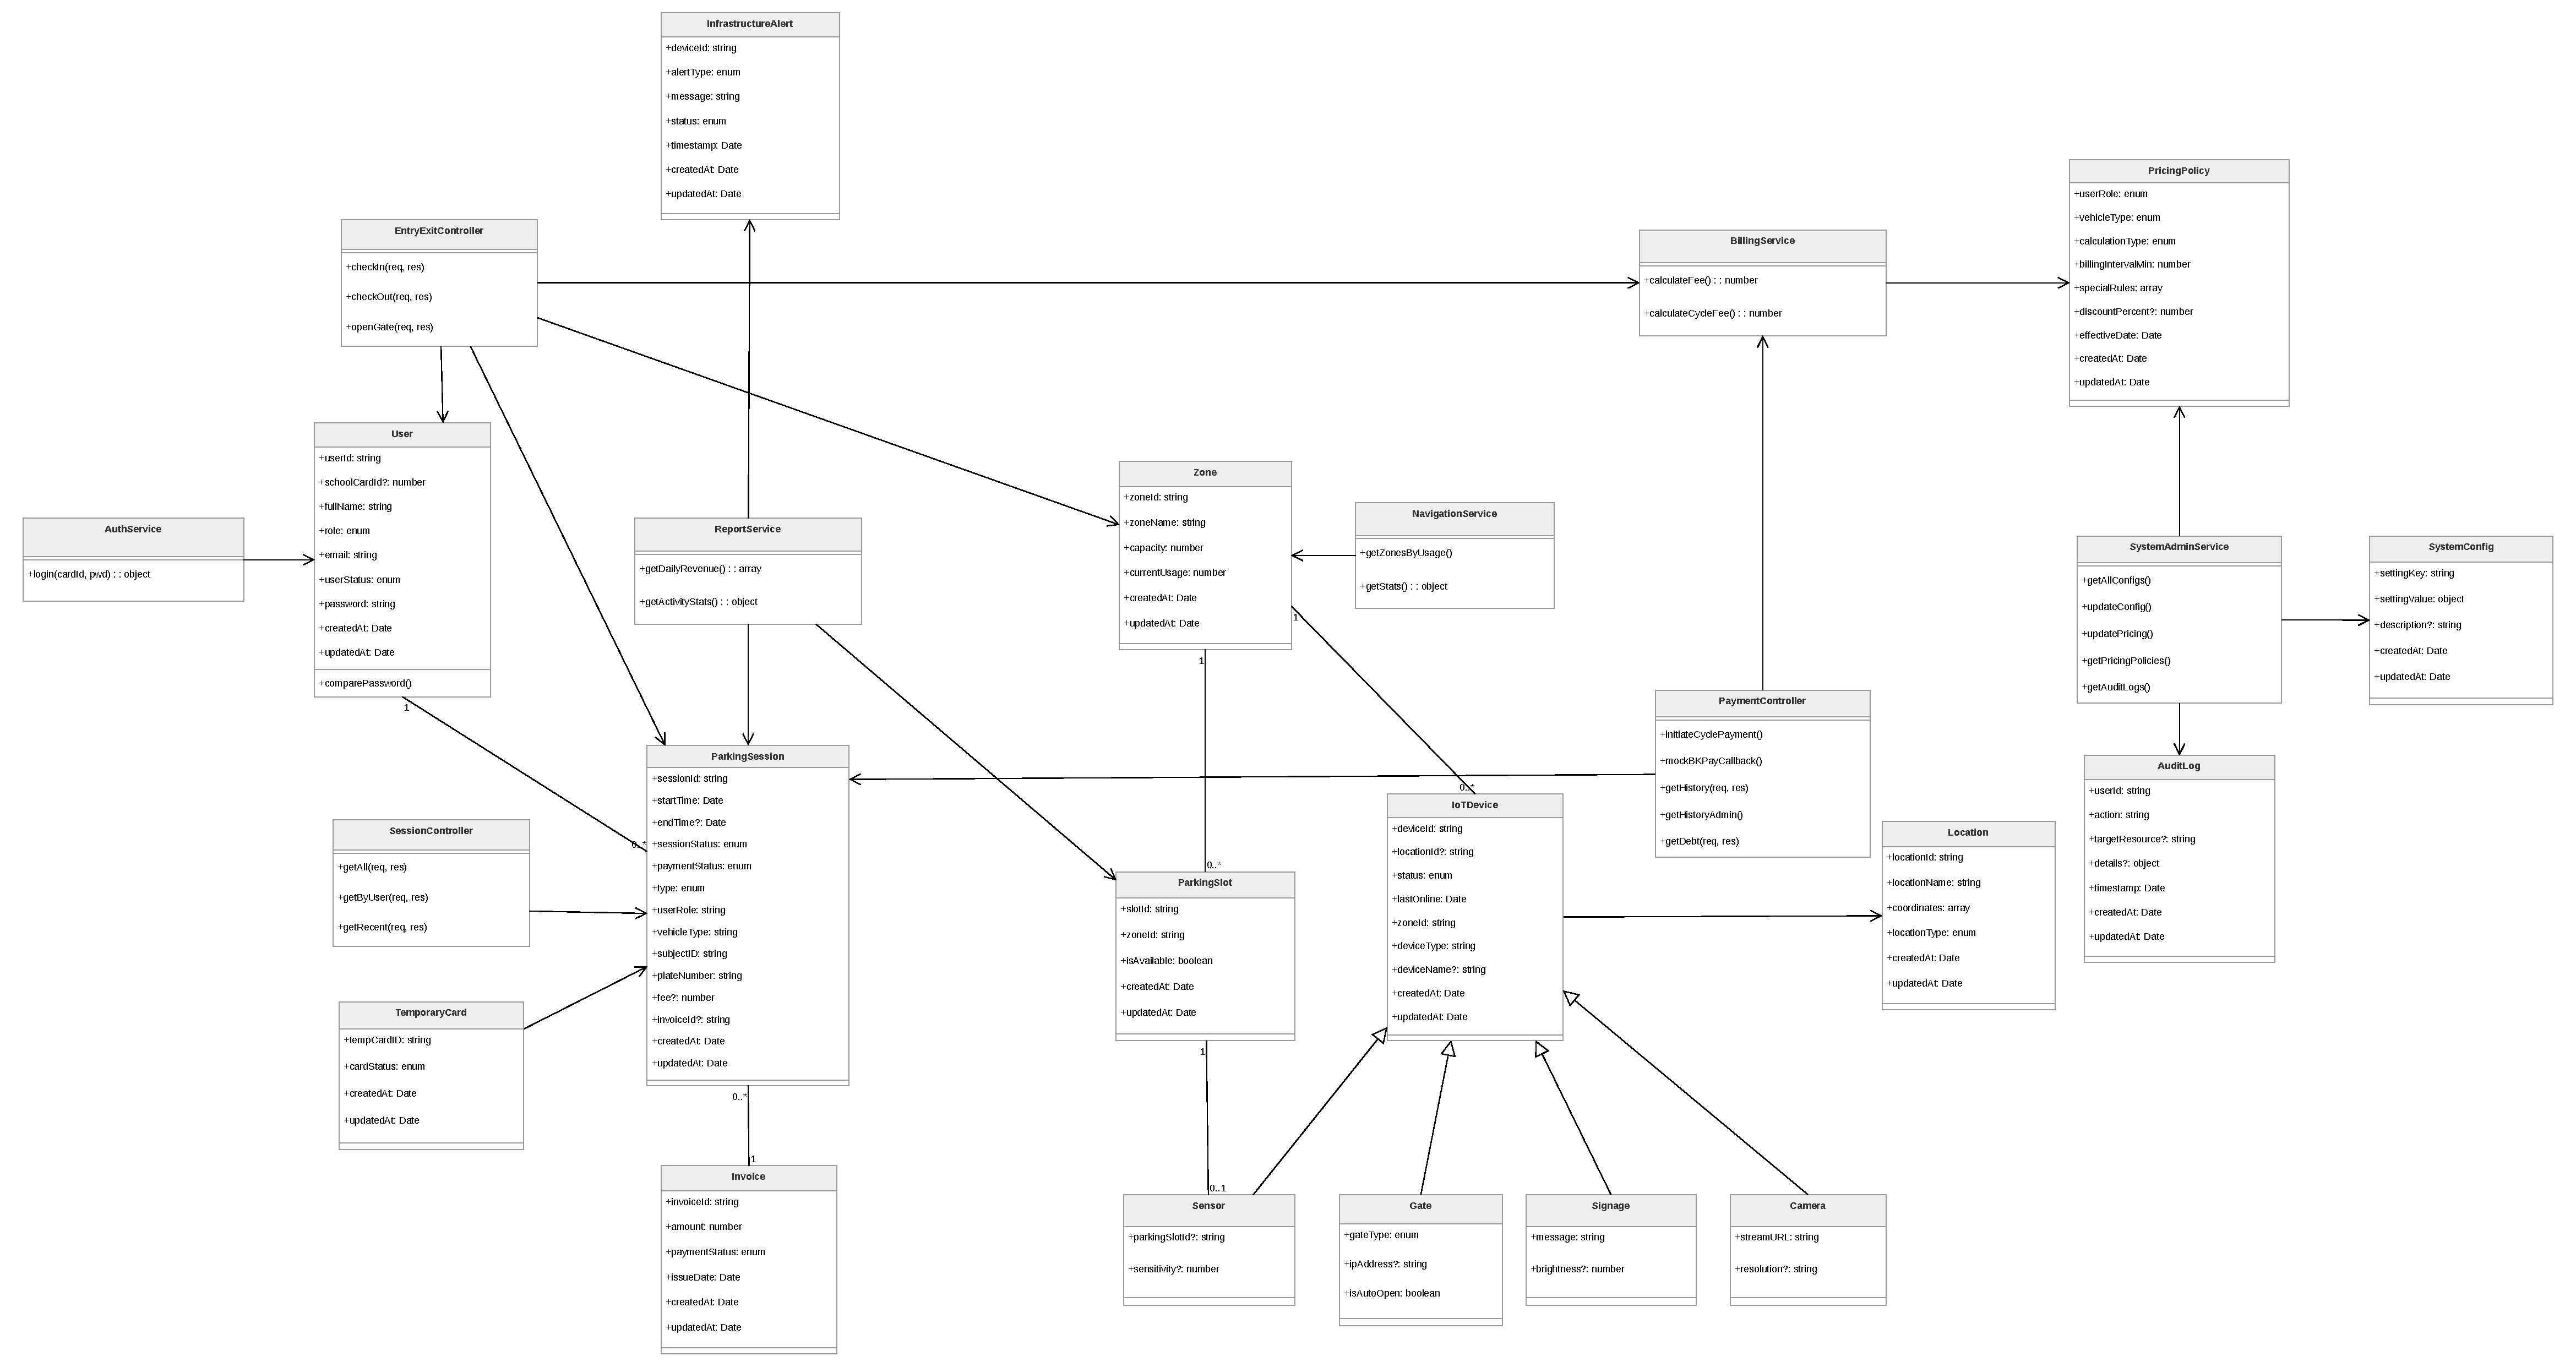
\includegraphics[width=\textwidth]{figures/class-diagram/class-diagram.pdf}
}
\caption{Complete Class Diagram - Smart Parking IoT System (Click to view full resolution)}
\label{fig:class-diagram}
\end{figure}

\subsection{Domain Model Classes}

The system uses a layered architecture with clear separation between data models, business logic, and API interfaces.

\subsubsection{Core Entities}
\begin{itemize}
\item \textbf{User:} Represents system users with authentication and role information
\item \textbf{ParkingSession:} Tracks individual parking sessions with timing and payment data
\item \textbf{Zone:} Defines parking zones with capacity management
\item \textbf{ParkingSlot:} Represents individual parking spaces within zones
\end{itemize}

\subsubsection{IoT and Infrastructure}
\begin{itemize}
\item \textbf{IoTDevice:} Abstract base class for all IoT devices (sensors, gates, signage, cameras)
\item \textbf{Sensor:} Parking space occupancy sensors
\item \textbf{Gate:} Entry/exit gate controllers
\item \textbf{Signage:} Dynamic display boards for guidance
\item \textbf{Camera:} Security and monitoring cameras
\end{itemize}

\subsubsection{Business Entities}
\begin{itemize}
\item \textbf{PricingPolicy:} Defines pricing rules based on user roles and vehicle types
\item \textbf{Invoice:} Financial transaction records
\item \textbf{TemporaryCard:} Guest access management
\end{itemize}

\subsubsection{Supporting Entities}
\begin{itemize}
\item \textbf{Location:} Geographic positioning data
\item \textbf{MappingConfig:} UI layout configuration for devices
\item \textbf{InfrastructureAlert:} System monitoring and alerts
\item \textbf{SystemConfig:} Application configuration settings
\item \textbf{AuditLog:} Security and compliance logging
\item \textbf{SystemLog:} Operational logging with TTL
\end{itemize}

\subsection{Service Layer Classes}

\subsubsection{Business Services}
\begin{itemize}
\item \textbf{AuthService:} Handles user authentication and JWT token management
\item \textbf{BillingService:} Calculates parking fees and manages payment processing
\item \textbf{NavigationService:} Provides zone utilization and statistics
\item \textbf{ReportService:} Generates business intelligence reports
\item \textbf{SystemAdminService:} Manages system configuration and policies
\item \textbf{SystemLogService:} Centralized logging and event emission
\end{itemize}

\subsection{Controller Layer Classes}

\subsubsection{API Controllers}
\begin{itemize}
\item \textbf{EntryExitController:} Manages parking session lifecycle (check-in/check-out)
\item \textbf{PaymentController:} Handles payment processing and billing cycles
\item \textbf{SessionController:} Provides session management and history APIs
\end{itemize}

\subsection{Frontend Types}

\subsubsection{UI Mapping Types}
\begin{itemize}
\item \textbf{PlacedDevice:} Represents devices positioned on the parking map
\item \textbf{CanvasTransform:} Handles map zooming and panning
\item \textbf{ParkingMap:} Complete map configuration with zones and devices
\end{itemize}

\subsection{Key Relationships}

\subsubsection{Inheritance Relationships}
\begin{itemize}
\item \textbf{IoTDevice} is the base class for Sensor, Gate, Signage, and Camera
\item Uses discriminator pattern in MongoDB for polymorphic storage
\end{itemize}

\subsubsection{Association Relationships}
\begin{itemize}
\item \textbf{User} creates multiple \textbf{ParkingSession} instances
\item \textbf{Zone} contains multiple \textbf{ParkingSlot} instances
\item \textbf{Zone} manages multiple \textbf{IoTDevice} instances
\item \textbf{ParkingSession} generates \textbf{Invoice} records
\end{itemize}

\subsubsection{Dependency Relationships}
\begin{itemize}
\item \textbf{Controllers} depend on \textbf{Services} for business logic
\item \textbf{Services} depend on \textbf{Models} for data access
\item \textbf{Frontend} depends on \textbf{Controllers} via REST APIs
\end{itemize}

\subsection{Design Patterns Applied}

\subsubsection{Structural Patterns}
\begin{itemize}
\item \textbf{Layered Architecture:} Clear separation between presentation, application, domain, and infrastructure
\item \textbf{Repository Pattern:} Models encapsulate data access logic
\item \textbf{Factory Pattern:} IoTDevice discriminator creates appropriate device types
\end{itemize}

\subsubsection{Behavioral Patterns}
\begin{itemize}
\item \textbf{Observer Pattern:} Event-driven updates for real-time monitoring
\item \textbf{Strategy Pattern:} PricingPolicy supports different calculation strategies
\item \textbf{Middleware Pattern:} Cross-cutting concerns handled by Express middleware
\end{itemize}

\subsection{Database Mapping}

\subsubsection{MongoDB Collections}
Each class maps to a MongoDB collection with the following naming convention:
\begin{itemize}
\item \textbf{users} - User documents
\item \textbf{parkingSessions} - ParkingSession documents
\item \textbf{zones} - Zone documents
\item \textbf{parkingSlots} - ParkingSlot documents
\item \textbf{iotDevices} - IoTDevice documents (with discriminator key)
\item \textbf{pricingPolicies} - PricingPolicy documents
\item \textbf{invoices} - Invoice documents
\end{itemize}

\subsubsection{Indexing Strategy}
\begin{itemize}
\item Compound indexes on frequently queried fields (userId + status, zoneId + isAvailable)
\item TTL indexes on SystemLog collection for automatic cleanup
\item Text indexes for search functionality
\end{itemize}

\subsubsection{Denormalization Strategy}
\begin{itemize}
\item Zone.currentUsage denormalized for fast capacity checks
\item User role information cached in ParkingSession for billing calculations
\item Pricing data embedded in calculation results to maintain historical accuracy
\end{itemize}